% Created 2020-05-17 Sun 13:39
% Intended LaTeX compiler: pdflatex
\documentclass[12pt]{report}
\usepackage[utf8]{inputenc}
\usepackage[T1]{fontenc}
\usepackage{graphicx}
\usepackage{grffile}
\usepackage{longtable}
\usepackage{wrapfig}
\usepackage{rotating}
\usepackage[normalem]{ulem}
\usepackage{amsmath}
\usepackage{textcomp}
\usepackage{amssymb}
\usepackage{capt-of}
\usepackage{hyperref}
\setlength{\parindent}{0pt}
\usepackage[margin=1in]{geometry}
\usepackage{emptypage}
\usepackage{tikz}
\usetikzlibrary{graphs,graphs.standard,bayesnet,arrows.meta,shapes.arrows}

% Colorlinks sets pdfborder to zero.
%\hypersetup{colorlinks,linkcolor=,urlcolor=gray}

%\usepackage[a4paper,top=2.25cm,bottom=2.25cm,left=3.0cm,right=3.0cm]{geometry}

%% arial font?????????
%% \usepackage[scaled]{uarial}
%% \renewcommand*\familydefault{\sfdefault} %% Only if the base font of the document is to be sans serif
%% \usepackage[T1]{fontenc}

\makeatletter
\renewenvironment{abstract}{%
    \if@twocolumn
      \section*{\abstractname}%
    \else %% <- here I've removed \small
      \begin{center}%
        {\bfseries \Huge\abstractname\vspace{\z@}}%  %% <- here I've added \Large
      \end{center}%
      \quotation
    \fi}
    {\if@twocolumn\else\endquotation\fi}
\makeatother

%\pagecolor{yellow!10}

\documentclass{book}
\usepackage{sectsty}
\chapternumberfont{\large} 
\chaptertitlefont{\huge}

\usepackage{hyperref}
\hypersetup{%
  colorlinks=false,% hyperlinks will be black
  linkbordercolor=red,% hyperlink borders will be red
  pdfborderstyle={/S/U/W 1}% border style will be underline of width 1pt
}

%% \usepackage[T1]{fontenc}
%% \usepackage{libertine}
%% \usepackage{graphicx}
%% \usepackage[svgnames]{xcolor}
%% \usepackage{framed}

%% \newcommand*\openquote{\makebox(25,-22){\scalebox{5}{``}}}
%% \newcommand*\closequote{\makebox(25,-22){\scalebox{5}{''}}}
%% \colorlet{shadecolor}{Azure}

%% \makeatletter
%% \newif\if@right
%% \def\shadequote{\@righttrue\shadequote@i}
%% \def\shadequote@i{\begin{snugshade}\begin{quote}\openquote}
%% \def\endshadequote{%
%%   \if@right\hfill\fi\closequote\end{quote}\end{snugshade}}
%% \@namedef{shadequote*}{\@rightfalse\shadequote@i}
%% \@namedef{endshadequote*}{\endshadequote}
%% \makeatother
%% \begin{document}


\author{Louis James}
\date{\today}
\title{Describing systems for the exploration of tangible and spatial computer interaction}
\hypersetup{
 pdfauthor={Louis James},
 pdftitle={Describing systems for the exploration of tangible and spatial computer interaction},
 pdfkeywords={},
 pdfsubject={Final year project for Creative Computing},
 pdfcreator={Emacs 26.3 (Org mode 9.3.6)}, 
 pdflang={English}}
\begin{document}

\maketitle

\renewcommand{\abstractname}{Acknowledgements}
\begin{abstract}
 Thanks to my family, Florent, Chudleigh dwellers, Jamie ...
\end{abstract}
\newpage

\renewcommand{\abstractname}{Abstract}
\begin{abstract}
Presented here is a specification of experimental approaches to computer
interaction based on spatial and tangible methods. The report describes an
prototypical implementation of a base system for interaction in space and a
theoretical API for such a system and similar systems. This utilises computer
vision techniques to analyse a surface to track objects and project onto the
space creating a feedback system for interaction. To finish a
ethnomethodological framework for evaluation and further development is
proposed???


\end{abstract}
\tableofcontents
\listoffigures
\chapter{Introduction}
\label{sec:orgc960828}

\section{Project aims}
\label{sec:orgde0f111}

\begin{itemize}
\item open source project for tangible interaction
\item Prototypical
\item ethnomethodological frameworks for evaluation
\end{itemize}

\chapter{Background}
\label{sec:org4525a2e}

The motivation for this project stems in part from a feeling of frustration in
 how working on computers can often be a constricted affair and a pondering over
 how we might expand the \emph{keyboard-mouse-monitor} model to improve the utility
 of computers regarding our own perceptive abilities. How might a spatial,
 haptic and tangible environment for interaction create an improved space for
 working and thinking with computers as well with our physical health? How might
 such an environment fundamentally augment our cognitive capabilities; memory
 and learning as well as creativity itself?

\section{Definitions}
\label{sec:org5649234}
\begin{enumerate}
\item Computing
\label{sec:orgee67d03}
\item keyboard-mouse-monitor model (kmm model) (?)
\label{sec:org8d933b3}
\item Cognition
\label{sec:org2acb25f}
\item Exocortex
\label{sec:org73f7ba7}
\end{enumerate}

\section{Beginning with the Exocortex}
\label{sec:orgecfdd8c}

I started off looking at \emph{Exocortexes} and other personal archiving systems.
Systems that allow the user to externalise thought and memory. This could be via
simply storing and organising work and ideas efficiently and methodically or
unifying many tasks or different workflows into a singular interface. \\

Org mode is a good example of such a system. Org mode is a "computing
environment for authoring mixed natural and computer language documents"
\cite{Schulte:Davison:Dye:Dominik:2011:JSSOBK:v46i03}. It is designed for taking
notes, producing documents and organising and runs inside of the text editor,
Emacs. It has the ability to export to different formats such as HTML, \LaTeX{} and
supports "outlining, note-taking, hyperlinks, spreadsheets, TODO lists, project
planning, GTD" as well as literate programming, all in plain-text
\cite{Schulte:Davison:Dye:Dominik:2011:JSSOBK:v46i03}. (it is incidentally what
this document is produced with) \\


Another point of reference when I was looking at externalised 'artificial
information-processing systems' was Devine Lu Linvega's Exocortex \href{https://wiki.xxiivv.com/site/nataniev.html}{XXIIV --
nataniev}. \emph{XXIIV} is a personal archive and log with documentation of Linvega's
personal tools and artworks. The site has gone through some changes since I
first came across it. Originally a static, javascript and lisp based website
with diaries, blog type posts and categorised personal logs. It is now somewhat
stripped back in style and has been rewritten in \href{https://en.wikipedia.org/wiki/C99}{C (C99)}. The work contains a
selection of esoteric programming tools including a synthetic language, games,
software all logged using their own \emph{Arvelie calendar} \cite{DevineNataniev}. \\

Both these two systems have their own specific use-cases, \emph{Org-mode}; in
academia and science and \emph{XXIIV}; an experimental personal archive. They both
utilise the contemporary and prevailing \emph{keyboard-mouse-monitor} paradigm
of computer interaction but push the boundaries of cognition in this medium,
particularly regarding memory and productivity. These two projects were a birth
point in thinking about how software systems can be augment thought and improve
learning ability and computer productivity.


\section{A virtual exploration of Dynamicland}
\label{sec:org4337574}

Another original and critical point of reference was \emph{Dynamicland}, a research
project in Oakland, USA. The aim of the project is to implement a new more
powerful and accessible model of computing.

\begin{quote}


In Oakland, we built the first full-scale realization of the vision, inviting
thousands of people into our space to collaborate. Together, these artists,
scientists, teachers, students, programmers, and non-programmers created
hundreds of projects that would have been impossible anywhere else.
-- Dynamicland.org 
\end{quote}


\emph{Dynamicland} is a communal computer where the building is the computer (ENIAC).
Programs are embodied in the room on pieces of colour-coded paper. The programs
are recognised via the codes and their code, stored in a database is then run,
it can also \emph{read} code using OCR but generally the code is there \href{https://thenewstack.io/dynamicland-rethinks-computer-interfaces/}{symbolically}.
Projectors on the ceiling transform the paper and workbenches into whatever the
programmer decides. This relatively simple model makes for an exciting new
ecosystem for collaborative computing and expressive programming. Victor
highlights his ideas for the progression of computing and interaction in a
series of talks (available online) and on his \href{http://worrydream.com}{website}. In his talk "Seeing
Spaces" he talks of a new kind of maker-space which allow makers to see across
time and possibilities. \emph{Dynamicland} offers a computational medium which allows
for full use of the human senses and a more \href{https://vimeo.com/115154289}{humane representation of thought}
\cite{VictorKayDynamicLand}. \\

\begin{figure}[htbp]
\centering
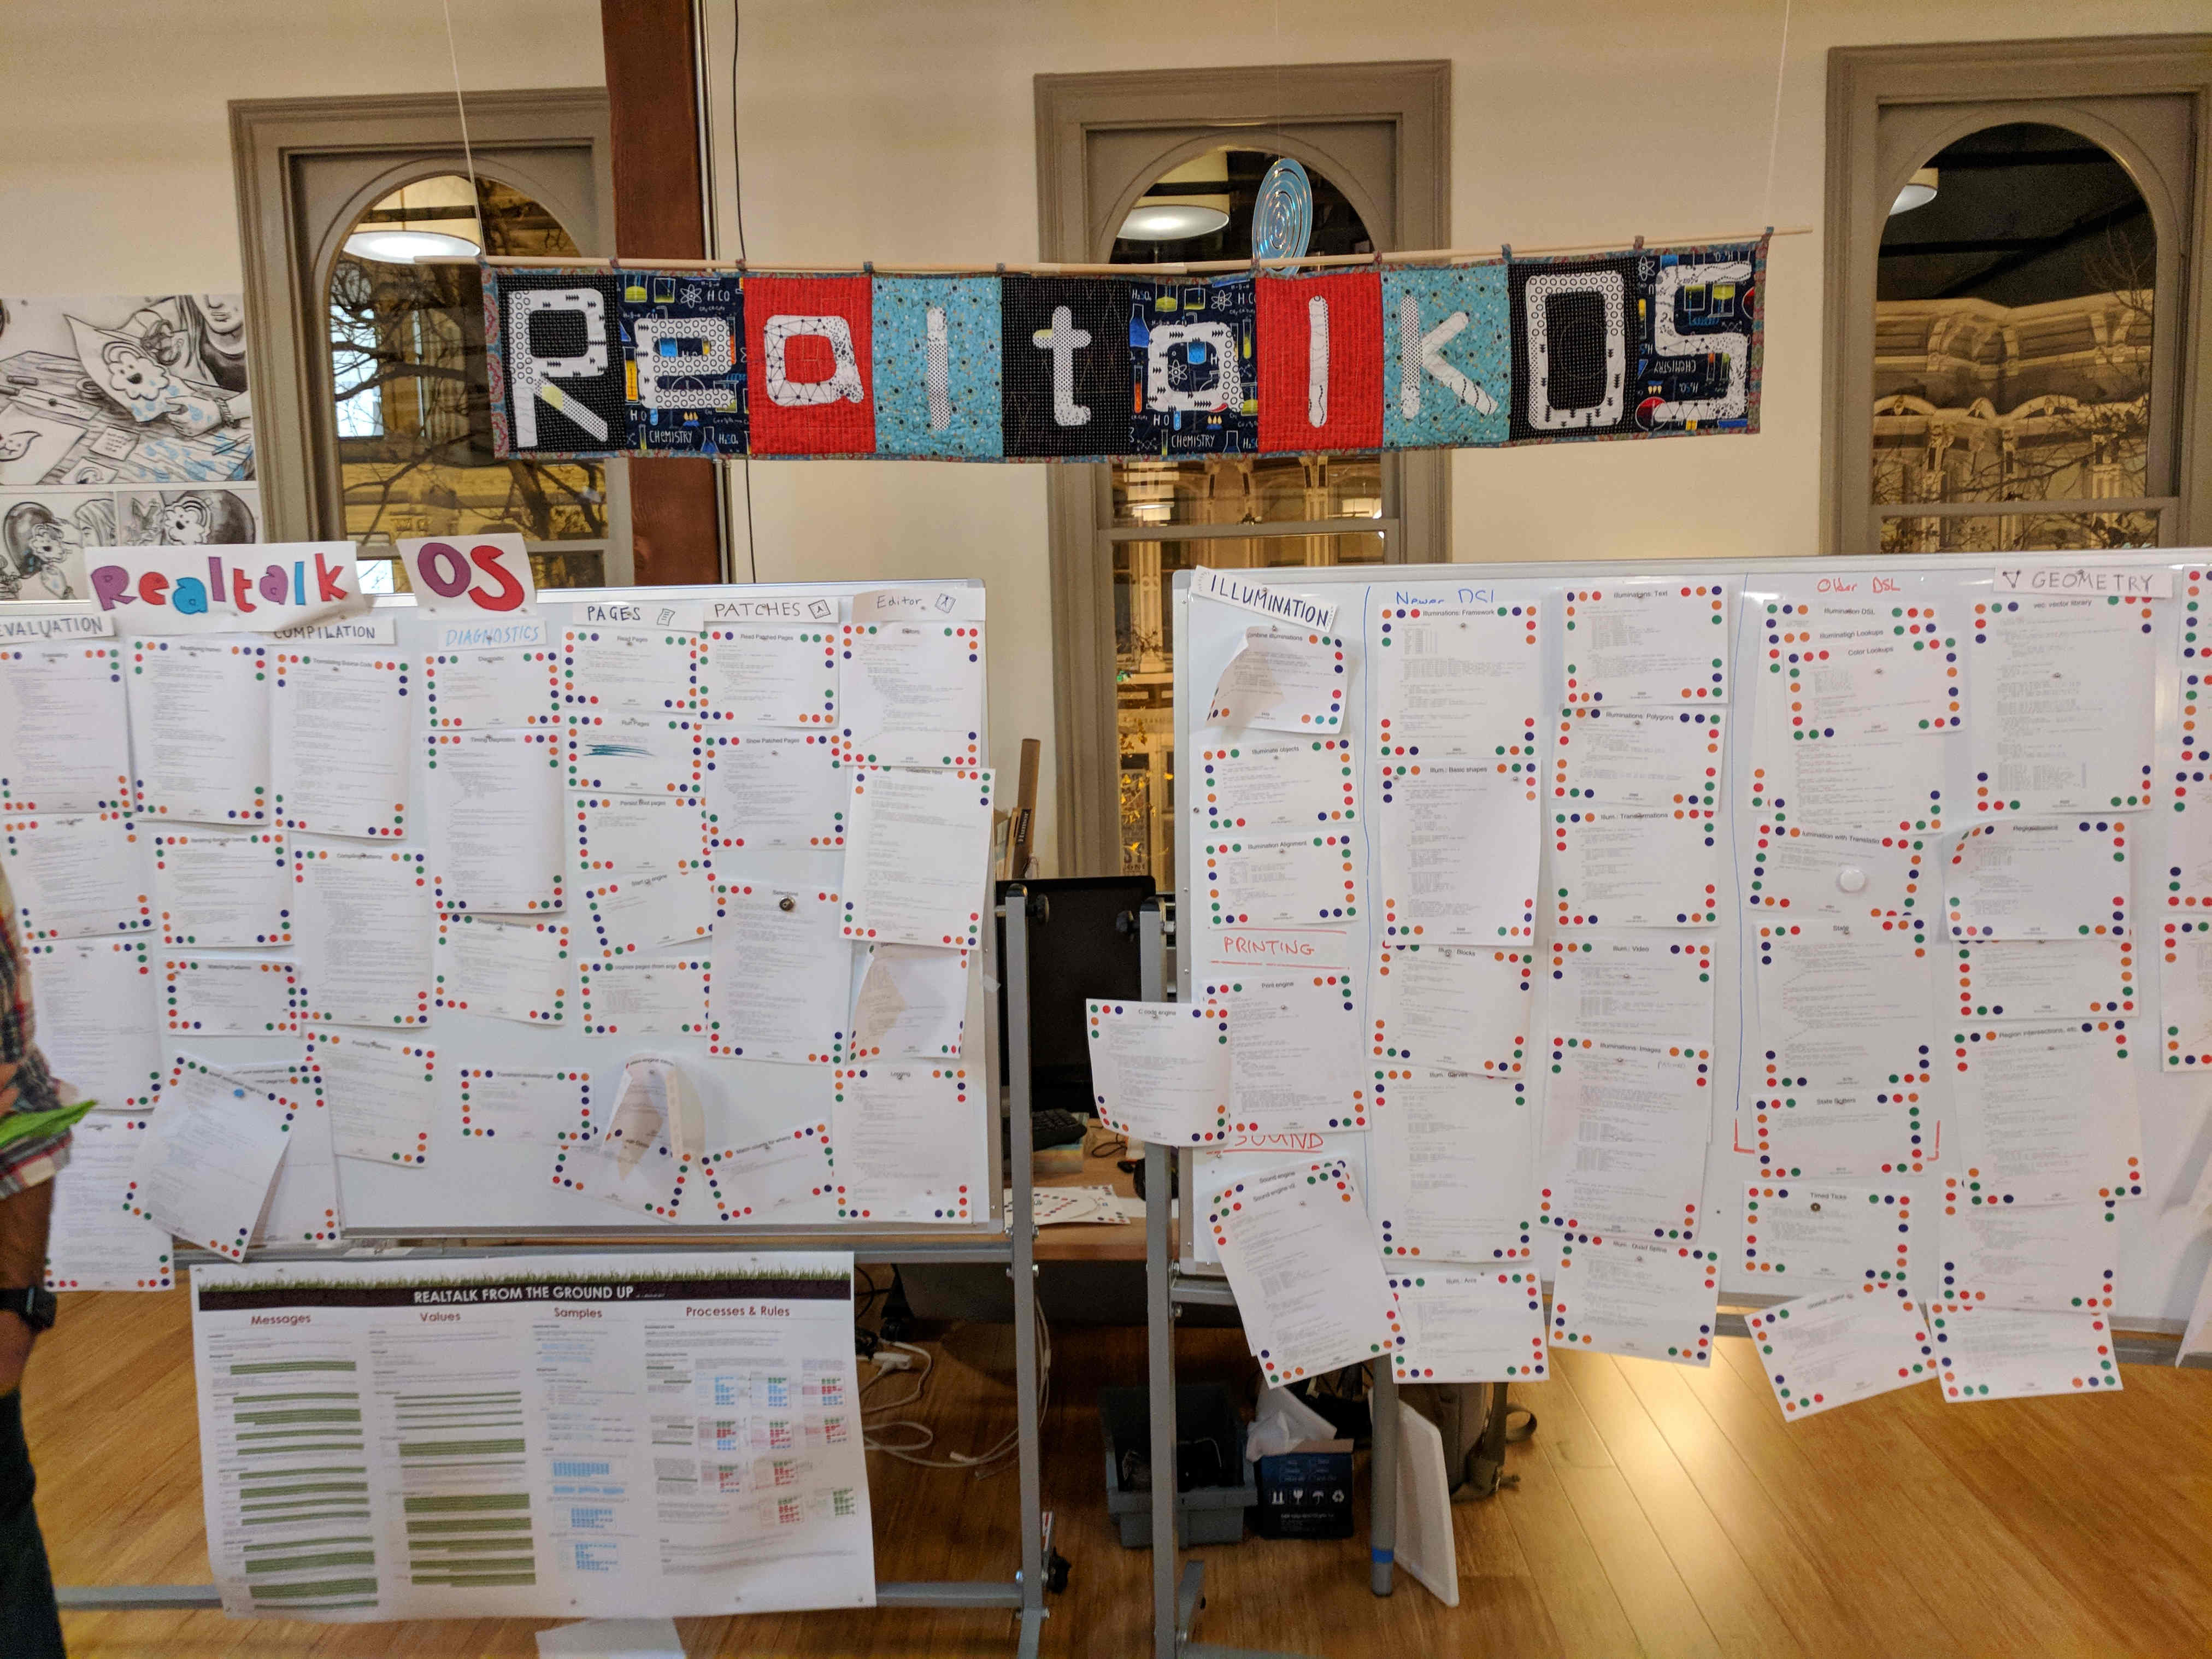
\includegraphics[width=12cm]{assets/realtalk-os.jpg}
\caption{RealtalkOS, the operating system of \emph{Dynamicland}}
\end{figure}  


\emph{DL} was the inspiration for the main physical and technical model for
this project, an \emph{augmented} workspace either on the floor or a table which is
projected onto. A camera/s pointing down onto the projection space is the sensor
for detecting interaction, with the projector as the actuator. This base model can be
seen in Figures \ref{pp-schema} and  \ref{systemSchema}.

\section{Paper programs - open source}
\label{sec:org2add96e}

Looking to find some of the code for \emph{Dynamicland} and a more detailed
specification of \textbf{DL} I stumbled across \emph{Paper Programs} (\emph{Dynamicland} has an
'open-source model', but it is only open if you can visit it physically as the
source code is physically in the space). \emph{Paper Programs} is a browser-based
partial clone of \emph{Dynamicland}. This was another starting point for playing
around with but I found that I couldn't set it up and have it stable enough to
develop on. It also suffers from being quite slow, due to the Computer Vision
and graphics being done in the browser (it uses a version of OpenCv compiled to
\href{https://webassembly.org/}{WebAssembly}) \cite{JpPaperPrograms}. While WebAssembly has the scope for doing
high-performance computation in the browser but I found there was still a
significant lag from detecting papers to projecting back down on to them.
Another branch which had implemented blob detection on the GPU I also found to
be slow and unstable (\href{https://github.com/janpaul123/paperprograms/pull/28}{Link to pull request}), this may have been due to my
lighting and camera setup.



\section{Sage digital research or Moving from implementation to abstraction}
\label{sec:orgaf13c1d}

Moving from implementation to abstraction

Ethnomethodology

Embodied Cognition

Haptic interfaces

\section{MIT Prof - tangible media group}
\label{sec:org23ad866}
\url{http://tangible.media.mit.edu/projects/}
\section{Nielsen: augmenting ltm and using ai to augment human-i ??????}
\label{sec:org8d8f366}

Other approaches to 

\cite{NielsenMich2018altm}

\cite{carter2017using}  

\section{Tangible bits - Hiroshi Ishii  and  Brygg Ullmer}
\label{sec:org8c86586}
\cite{IshiiH2002Tbdt}

\chapter{Specification and context}
\label{sec:org33acc38}

As in my original specification the main aim was to create a system for spatial
interaction. Initially I imagined it to work on a table top surface (in the end
it was developed on a floor mat due to considerations in my development
environment; see Chapter \ref{projectindepth}). The other principle component was
to that interaction would be based on the placement and movement of objects
around the work-surface. The position and movements of theses objects would be
picked up by a camera and actuated by a projector; both situated above the
surface looking down onto it. It could also be setup in a horizontal direction,
with, for example, magnetised components keeping the objects to a board.
Alongside this a computer keyboard may be used for additional input such as
inputting text or selecting something. \\

My original plan was to use the already made \emph{Paperprograms} system and build on
top of this. Due to technical issues with PP I decided to implement the system
myself using openFrameworks, a C++ toolkit for experimental application
development. I chose this framework as it has straightforward 'out of the box'
graphics capabilities as well as numerous Add-ons which include \emph{Opencv}
\cite{opencv_library} wrappers and GUI libraries as well as an active community of
users. This combination in one framework seemed suitable for quick
experimentation and prototyping for the project. The physical setup would
include a Projector and HD webcam and computer for running the application. \\

Another design consideration I had in mind was accessibility. From my research
into similar projects an aim was to create a similar system that could be open
source and easily setup so that others could build on top of the system. This
was another reason for using \href{https://openframeworks.cc/download/}{openFrameworks} which is cross platform (Windows,
OSx, IOS and Linux). This would mean with minor or no modification of the code,
it could be run on any all the major desktop platforms. The hardware
requirements are also the kind which are either cheaply sourced or available in
most educational institutions: one of the target areas that further development
was envisioned.



\begin{figure}[htbp]
\centering
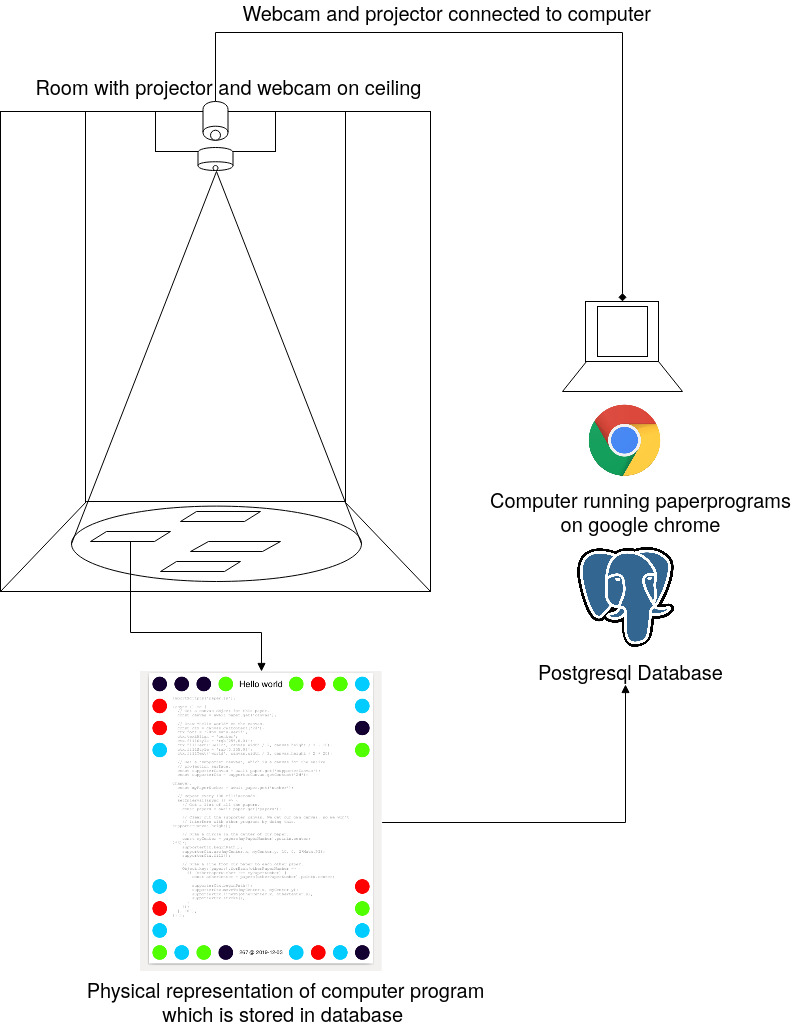
\includegraphics[width=15cm]{assets/pp-diag.png}
\caption{The initial physical schema: \emph{Paperprograms} \label{pp-schema}}
\end{figure}



\chapter{Project in depth \label{projectindepth}}
\label{sec:org34ac07c}

See system schema Fig.  

\begin{figure}[htbp]
\centering
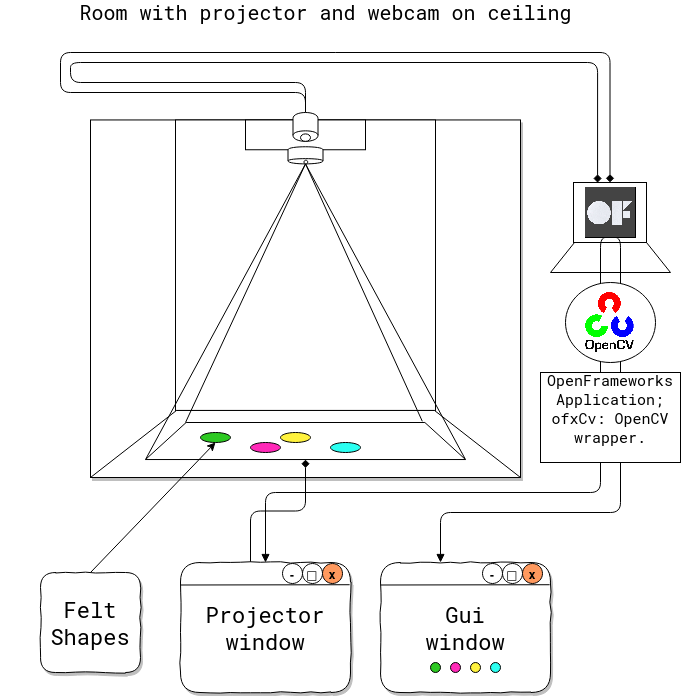
\includegraphics[width=15cm]{assets/project-schema-final.png}
\caption{System schema \label{systemSchema}}
\end{figure}

\section{Raspberry pi testing}
\label{sec:orgc3cf169}

\section{Build}
\label{sec:orgb218202}

\section{API}
\label{sec:org8660844}

\section{}
\label{sec:orgec11ad0}

\chapter{Creative process}
\label{sec:org477ac17}
\chapter{Debugging and problem solving}
\label{sec:org7bf93f5}
\chapter{Evaluation and Conclusions}
\label{sec:orgf7a68da}
\bibliographystyle{ieeetr} 
\bibliography{references}
\end{document}
